\documentclass{article}

\usepackage[margin=1in]{geometry}
\usepackage{amsmath,amsthm,amssymb}
\usepackage{bbm,enumerate,mathtools}
\usepackage{tikz}

\newenvironment{question}{\begin{trivlist}\item[\textbf{Question.}]}{\end{trivlist}}
\newenvironment{note}{\begin{trivlist}\item[\textbf{Note.}]}{\end{trivlist}}
\newenvironment{related}{\begin{trivlist}\item[\textbf{Related.}]\end{trivlist}\begin{enumerate}}{\end{enumerate}}
\begin{document}

\title{Problem 2.}
\date{}
\author{}
\maketitle

Jeremy Kun gives a canonical bijection between $\binom{n + 1}{2}$ and a discrete
tringle of length $n$, as seen in Figure 1.
\begin{figure}[!h]
  \centering
  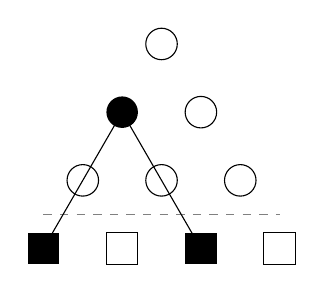
\begin{tikzpicture}
    \draw (1.5, 3 * 0.866) circle (0.2cm);
    \fill (1,2 * 0.866) circle (0.2cm);    \draw (2, 2 * 0.866) circle (0.2cm);
    \draw (0.5,0.866) circle (0.2cm);      \draw (1.5,0.866) circle (0.2cm);     \draw (2.5,0.866) circle (0.2cm);
    \draw[gray, dashed] (0, 0.5 * 0.866) -- (3, 0.5 * 0.866);
    \fill (-0.2,-0.2) rectangle (0.2,0.2); \draw (0.8,-0.2) rectangle (1.2,0.2); \fill (1.8,-0.2) rectangle (2.2,0.2); \draw (2.8,-0.2) rectangle (3.2,0.2);

    \draw (1,2 * 0.866) -- (0, 0);
    \draw (1,2 * 0.866) -- (2, 0);
  \end{tikzpicture}
  \caption{Bijection that maps a point on the triangle with side length 3 to a 2-subset of [3 + 1].}
\end{figure}

\begin{question}
  Is there a similar ``projection'' that bijects a point on the discrete
  tetrahedron to a \linebreak
  3-subset of [n + 2]?
\end{question}

\begin{note}
  Misha Lavrov gives a potential function to the question on Math Stack Exchange. \\
  (https://math.stackexchange.com/a/2468687/121988)
\end{note}

\begin{related}
  \item More generally is there a bijection from the $k$-simplex to a $k$-subset of [n + k - 1]?
\end{related}

\end{document}
